% !TeX spellcheck = de_CH_frami

\section{Graph Spektralanalyse\label{sec:sgwt:spectralanalysis}}
\rhead{Graph Spektralanalyse}

Nachdem wir nun die Grundlagen von Graphen und den Laplace Operator sowie die 
Laplace Matrix angeschaut haben, wollen wir uns nun der Spektralanalyse eines 
Graphen widmen.

\subsection{Laplace Matrix Eigenwerte}

Wenn man vom Spektrum eines Graphen spricht, meint man damit die Eigenwerte 
$\lambda$ seiner Laplace Matrix. Da diese Matrix bei einem ungerichteten 
Graphen immer symmetrisch ist, werden die daraus folgenden Eigenwerte und 
Eigenfunktionen auch immer real und gr\"osser gleich $0$ sein. Es gilt somit
\begin{equation}
0 = \lambda_0 < \lambda_1 \leq \lambda_2 \leq \cdots \leq \lambda_{N-1}.
\label{eq:sgwt:lambda:series}
\end{equation}
\Cref{fig:sgwt:lambda:line} zeigt die Eigenwerte $\lambda_0$ bis 
$\lambda_{999}$ eines Ringraphen mit 1000 Knoten.

\begin{figure}
    \centering
    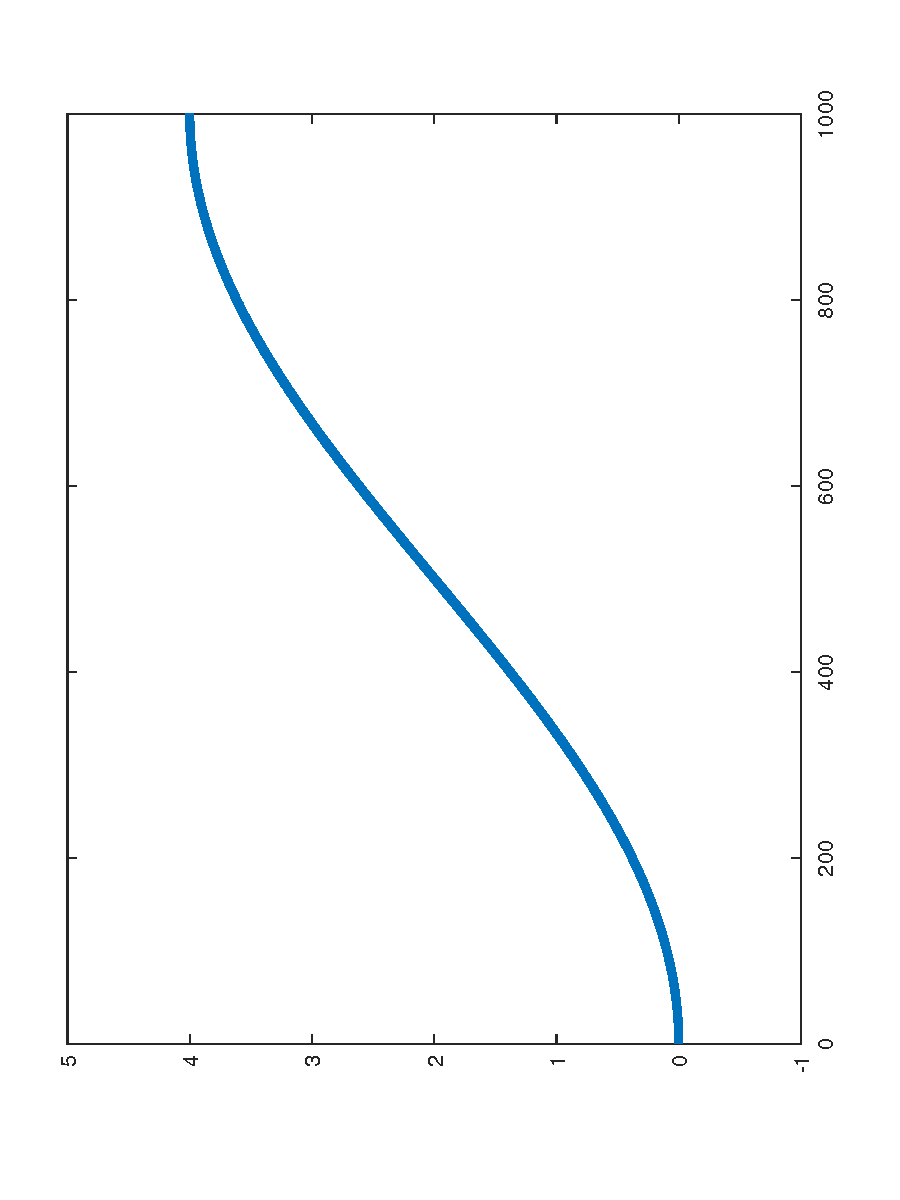
\includegraphics[
    angle=-90,
    origin=c,
    scale=0.6
    ]{papers/sgwt/images/ring-lambda.pdf}
    \vspace{-70pt}
    \caption{$\lambda_0$ bis $\lambda_{999}$ eines nicht gewichteten Ringraphen.
        \label{fig:sgwt:lambda:line}}
\end{figure}

\subsection{Laplace Matrix Eigenvektoren}

Eine weitere wichtige Rolle spielen die Eigenvektoren der Laplace Matrix. Diese 
sind n\"amlich approximierte Eigenfunktionen des Laplace Operators $\Delta$. So 
ist die komplexe Exponentialfunktion $e^{i\omega x}$ die Eigenfunktion des 
eindimensionalen Laplace Operators 
$\frac{d^2}{dx^2}$~\cite{chung_spectral_nodate}. Dies wird deutlich, wenn 
wir die Eigenfunktionen eines 
Ring-,~\cref{fig:sgwt:chi:ring0,fig:sgwt:chi:ring1,fig:sgwt:chi:ring2,fig:sgwt:chi:ring3,fig:sgwt:chi:ring4,fig:sgwt:chi:ring5},
oder 
Liniengraphen,~\cref{fig:sgwt:chi:line0,fig:sgwt:chi:line1,fig:sgwt:chi:line2,fig:sgwt:chi:line3,fig:sgwt:chi:line4,fig:sgwt:chi:line5},
darstellen. Auch die Kugelfunktionen $Y^m_l$, lassen mit den Hilfe der 
Eigenfunktionen eines Kugelgraphen approximieren, wie man 
in~\cref{fig:sgwt:chi:sphere} sehen kann. Dabei wird aber auch deutlich, dass 
diese Approximation nicht \"uberall gleich gut ist. Insbesondere dadurch, dass 
der Grad an den Polen stark von den anderen Knoten abweicht, findet dort eine 
Verzerrung statt.

\begin{figure}
\centering
\begin{minipage}[b]{0.49\textwidth}
    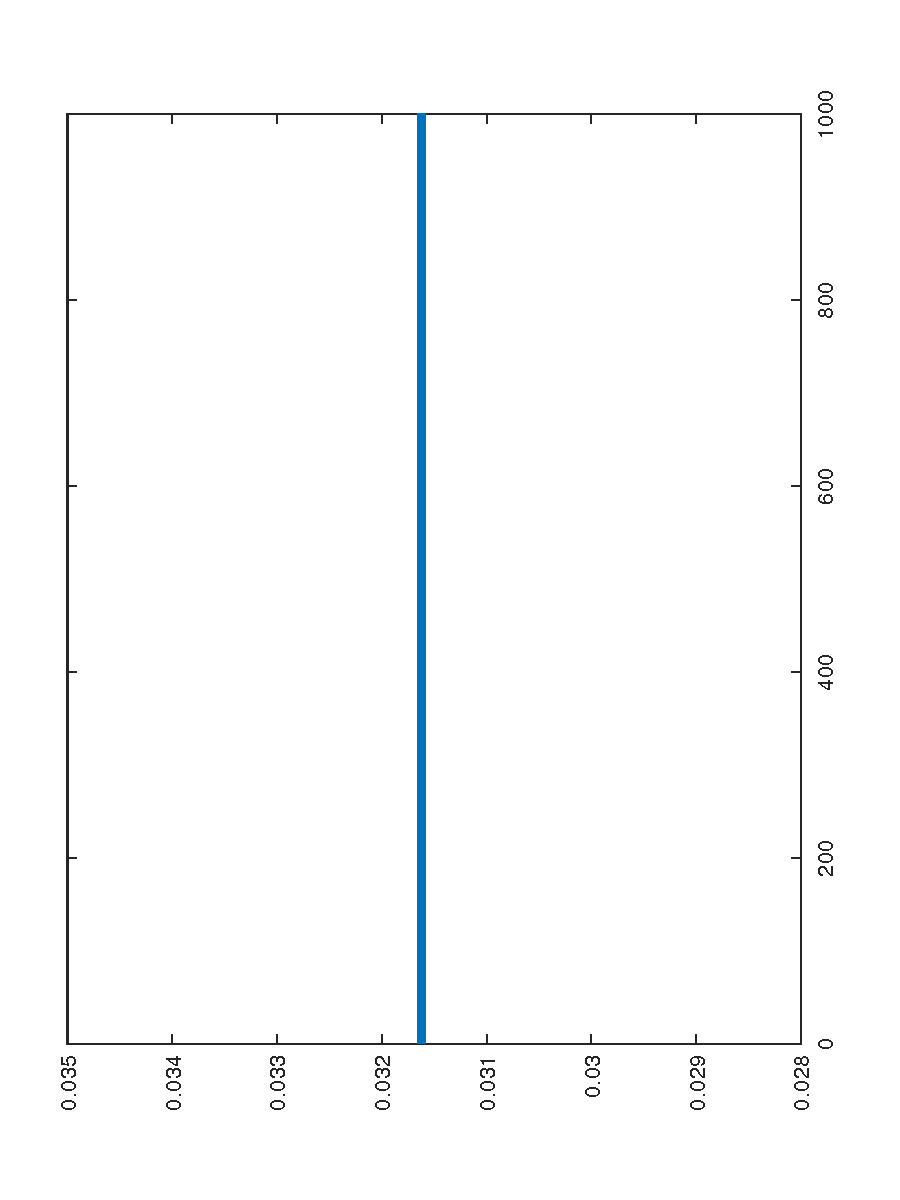
\includegraphics[
    angle=-90,
    origin=c,
    width=\textwidth]{papers/sgwt/images/ring-chi-1.pdf}
    \vspace{-45pt}
    \caption{$\chi_0$ eines ungewichteten Ringraphen mit 1000 Knoten.}
    \label{fig:sgwt:chi:ring0}
\end{minipage}
~
\begin{minipage}[b]{0.49\textwidth}
    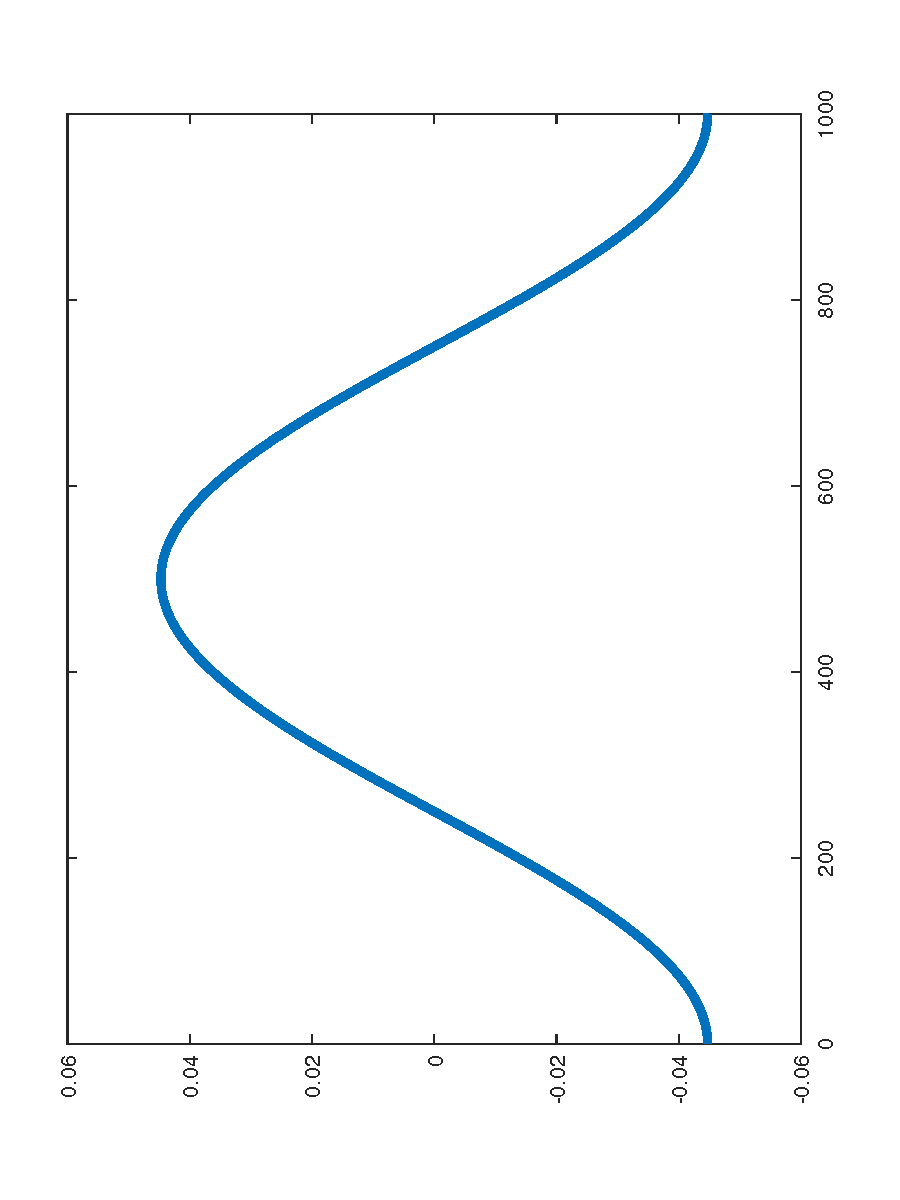
\includegraphics[
    angle=-90,
    origin=c,
    width=\textwidth]{papers/sgwt/images/ring-chi-2.pdf}
    \vspace{-45pt}
    \caption{$\chi_1$ eines ungewichteten Ringraphen mit 1000 Knoten.}
    \label{fig:sgwt:chi:ring1}
\end{minipage}
~
\begin{minipage}[b]{0.49\textwidth}
    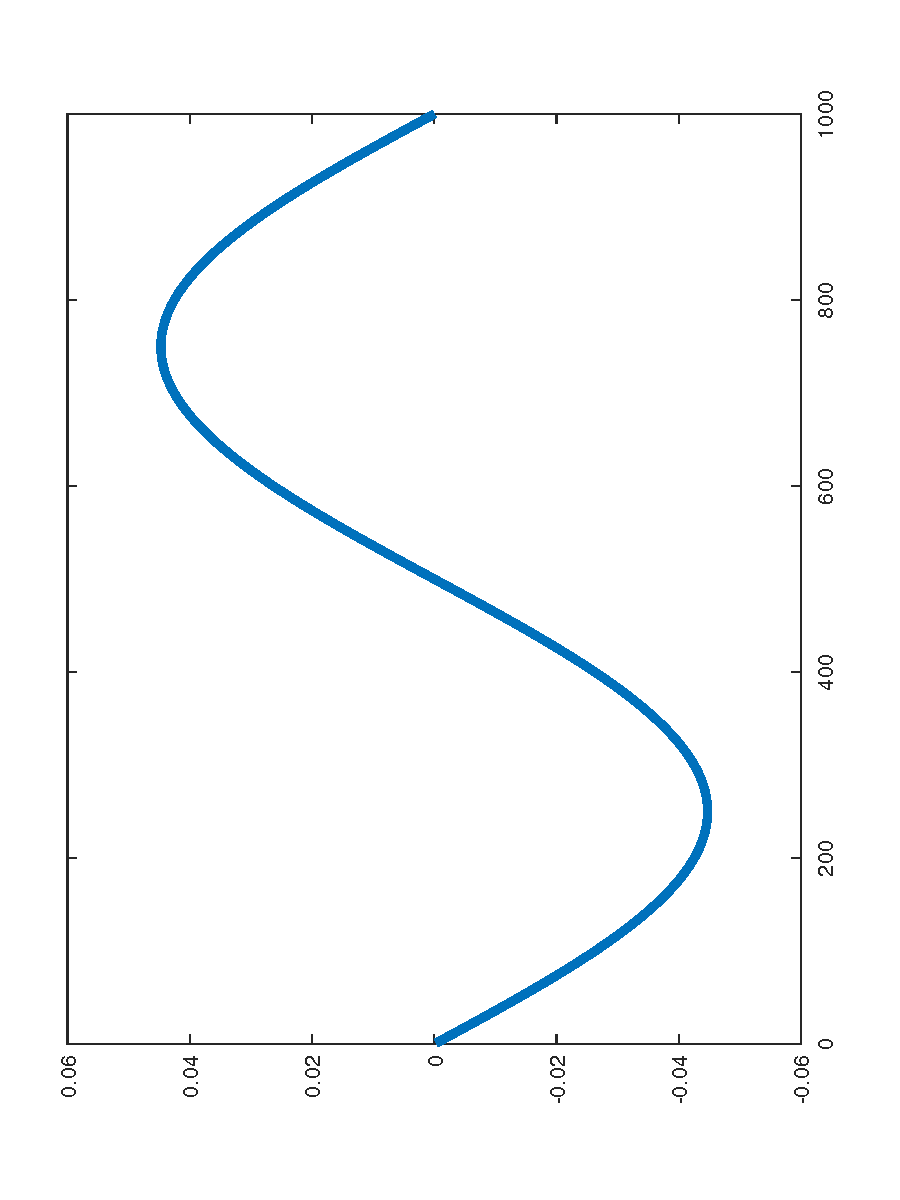
\includegraphics[
    angle=-90,
    origin=c,
    width=\textwidth]{papers/sgwt/images/ring-chi-3.pdf}
    \vspace{-45pt}
    \caption{$\chi_2$ eines ungewichteten Ringraphen mit 1000 Knoten.}
    \label{fig:sgwt:chi:ring2}
\end{minipage}
~
\begin{minipage}[b]{0.49\textwidth}
    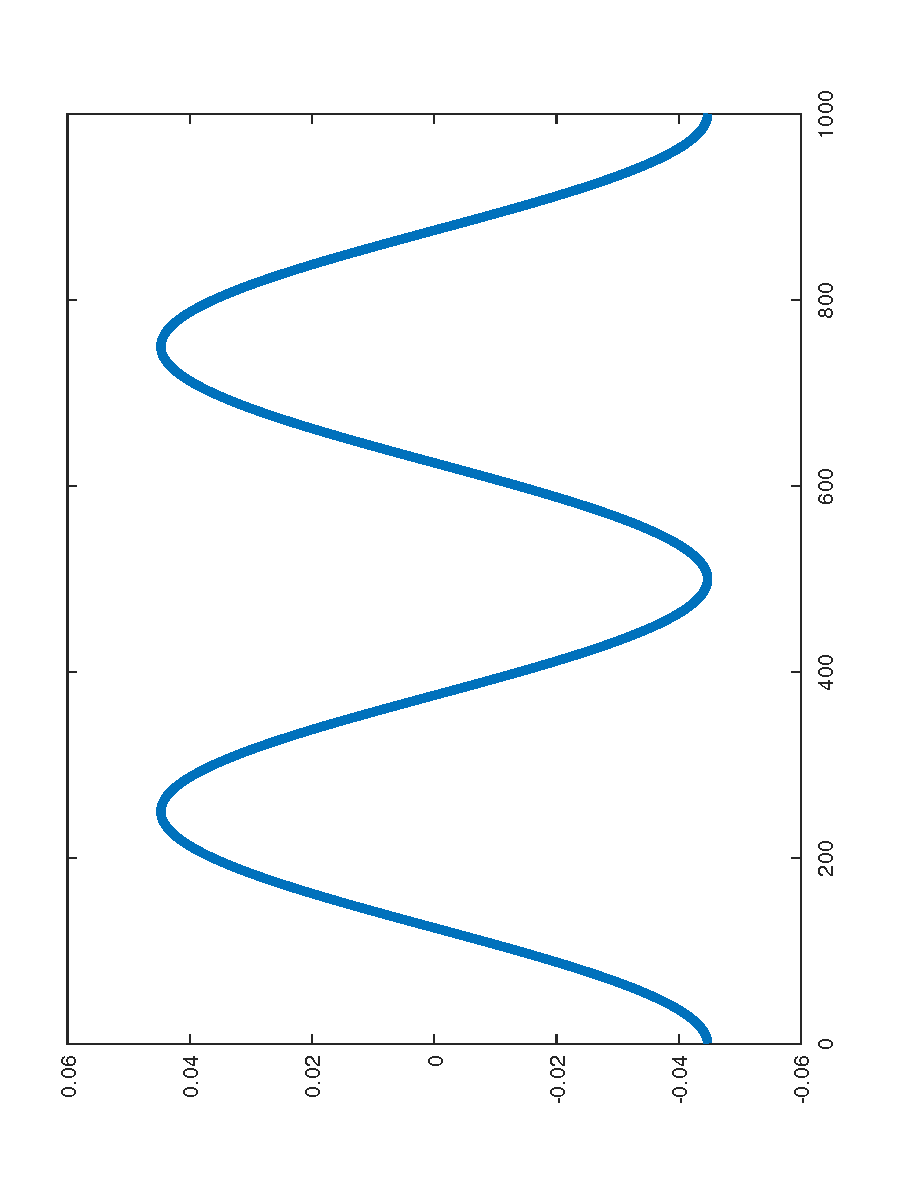
\includegraphics[
    angle=-90,
    origin=c,
    width=\textwidth]{papers/sgwt/images/ring-chi-4.pdf}
    \vspace{-45pt}
    \caption{$\chi_3$ eines ungewichteten Ringraphen mit 1000 Knoten.}
    \label{fig:sgwt:chi:ring3}
\end{minipage}
~
\begin{minipage}[b]{0.49\textwidth}
    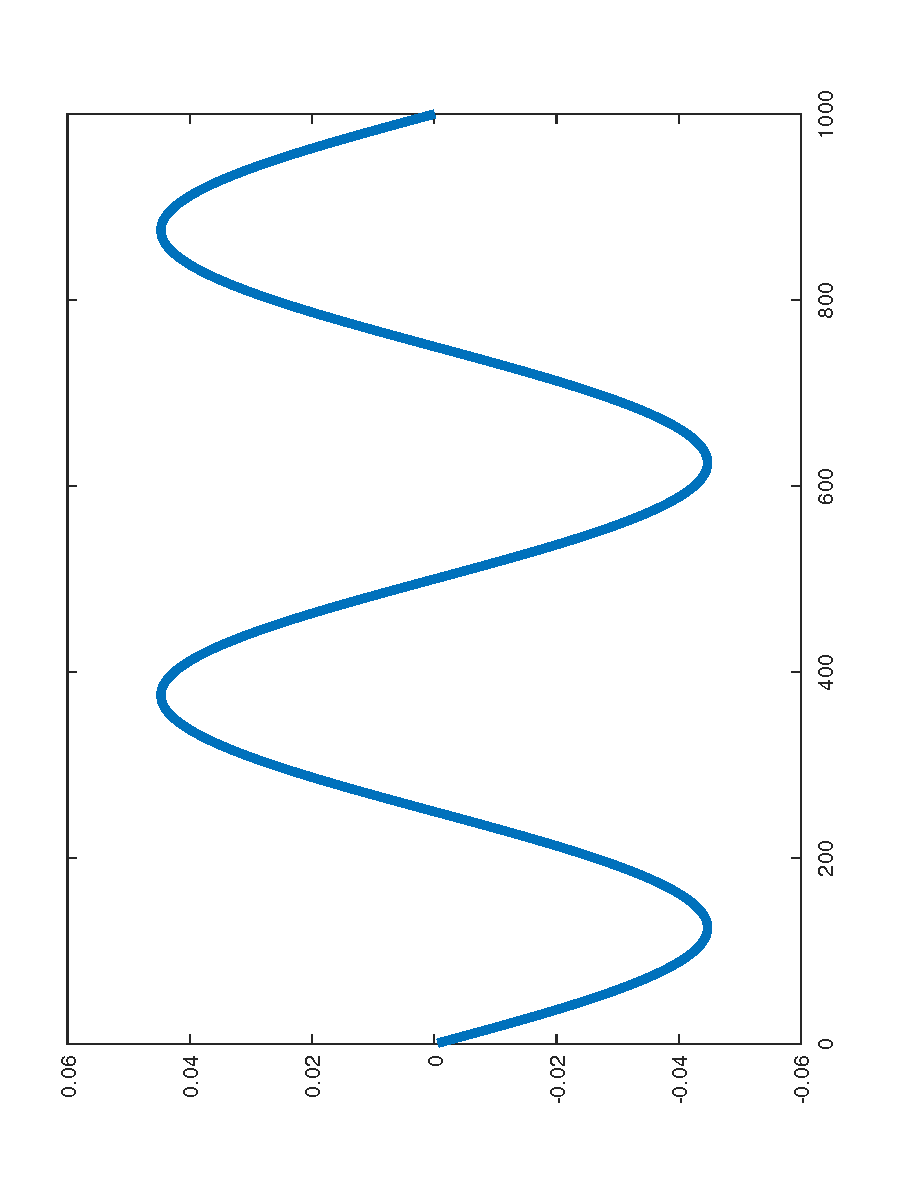
\includegraphics[
    angle=-90,
    origin=c,
    width=\textwidth]{papers/sgwt/images/ring-chi-5.pdf}
    \vspace{-45pt}
    \caption{$\chi_4$ eines ungewichteten Ringraphen mit 1000 Knoten.}
    \label{fig:sgwt:chi:ring4}
\end{minipage}
~
\begin{minipage}[b]{0.49\textwidth}
    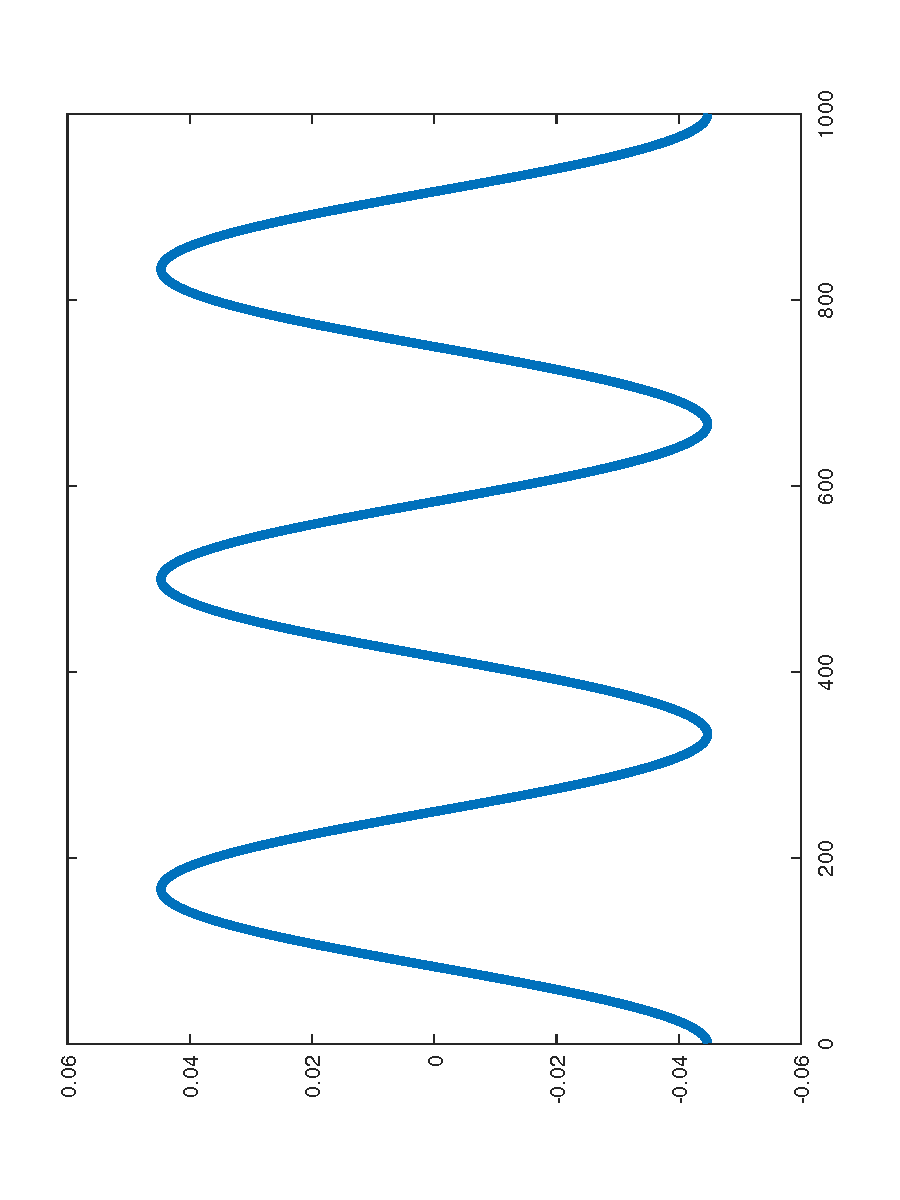
\includegraphics[
    angle=-90,
    origin=c,
    width=\textwidth]{papers/sgwt/images/ring-chi-6.pdf}
    \vspace{-45pt}
    \caption{$\chi_5$ eines ungewichteten Ringraphen mit 1000 Knoten.}
    \label{fig:sgwt:chi:ring5}
\end{minipage}
\end{figure}

\begin{figure}
    \centering
    \begin{minipage}[b]{0.49\textwidth}
        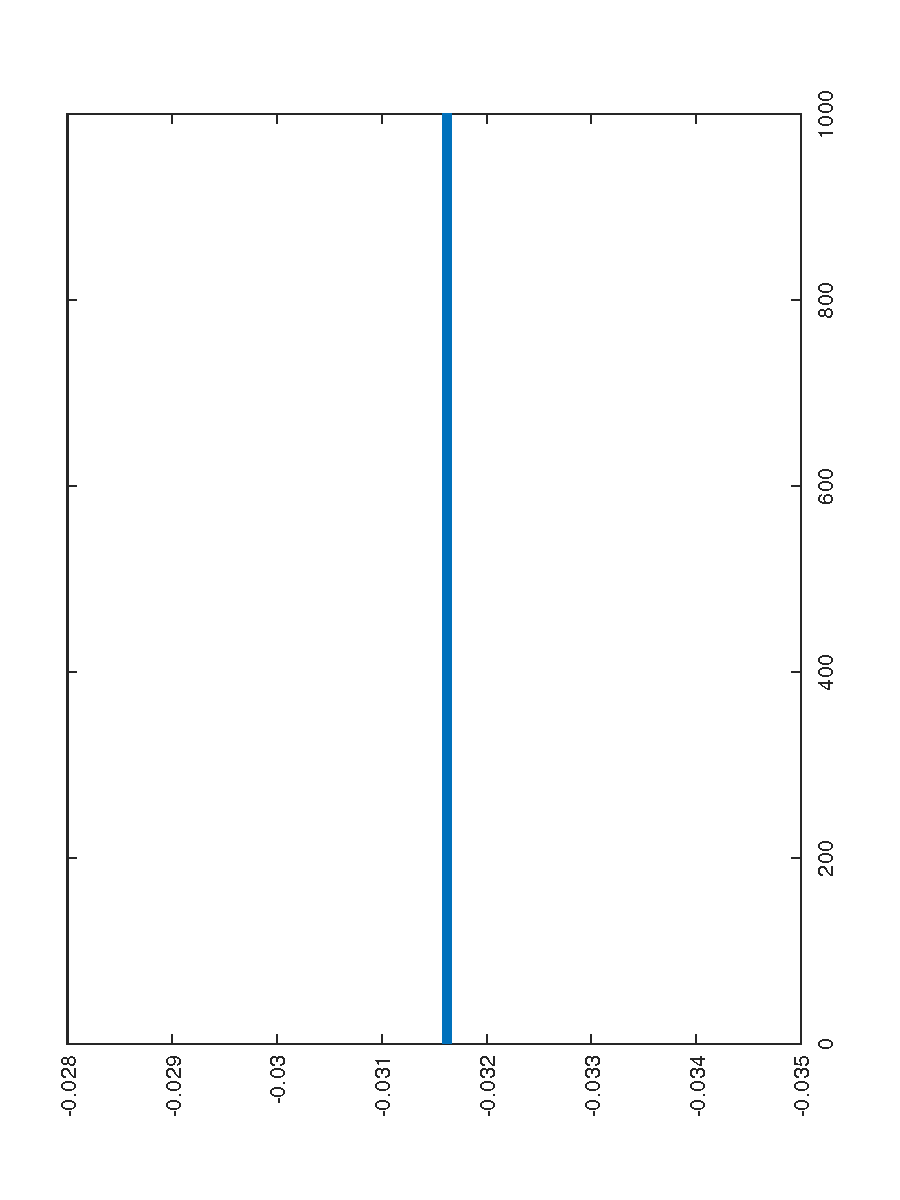
\includegraphics[
        angle=-90,
        origin=c,
        width=\textwidth]{papers/sgwt/images/line-chi-1.pdf}
        \vspace{-45pt}
        \caption{$\chi_0$ eines ungewichteten Liniengraphen mit 1000 
        Knoten.}
        \label{fig:sgwt:chi:line0}
    \end{minipage}
    ~
    \begin{minipage}[b]{0.49\textwidth}
        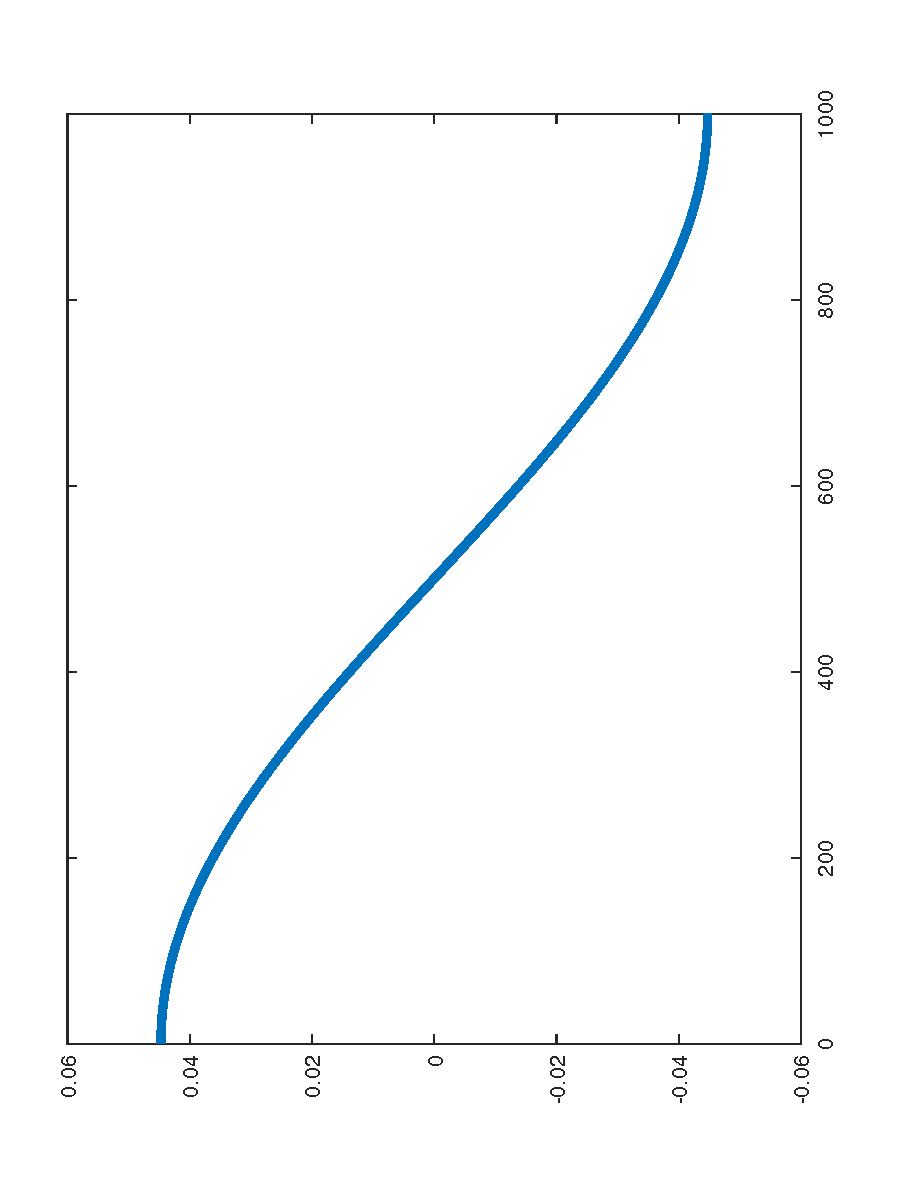
\includegraphics[
        angle=-90,
        origin=c,
        width=\textwidth]{papers/sgwt/images/line-chi-2.pdf}
        \vspace{-45pt}
        \caption{$\chi_1$ eines ungewichteten Liniengraphen mit 1000 
        Knoten.}
        \label{fig:sgwt:chi:line1}
    \end{minipage}
    ~
    \begin{minipage}[b]{0.49\textwidth}
        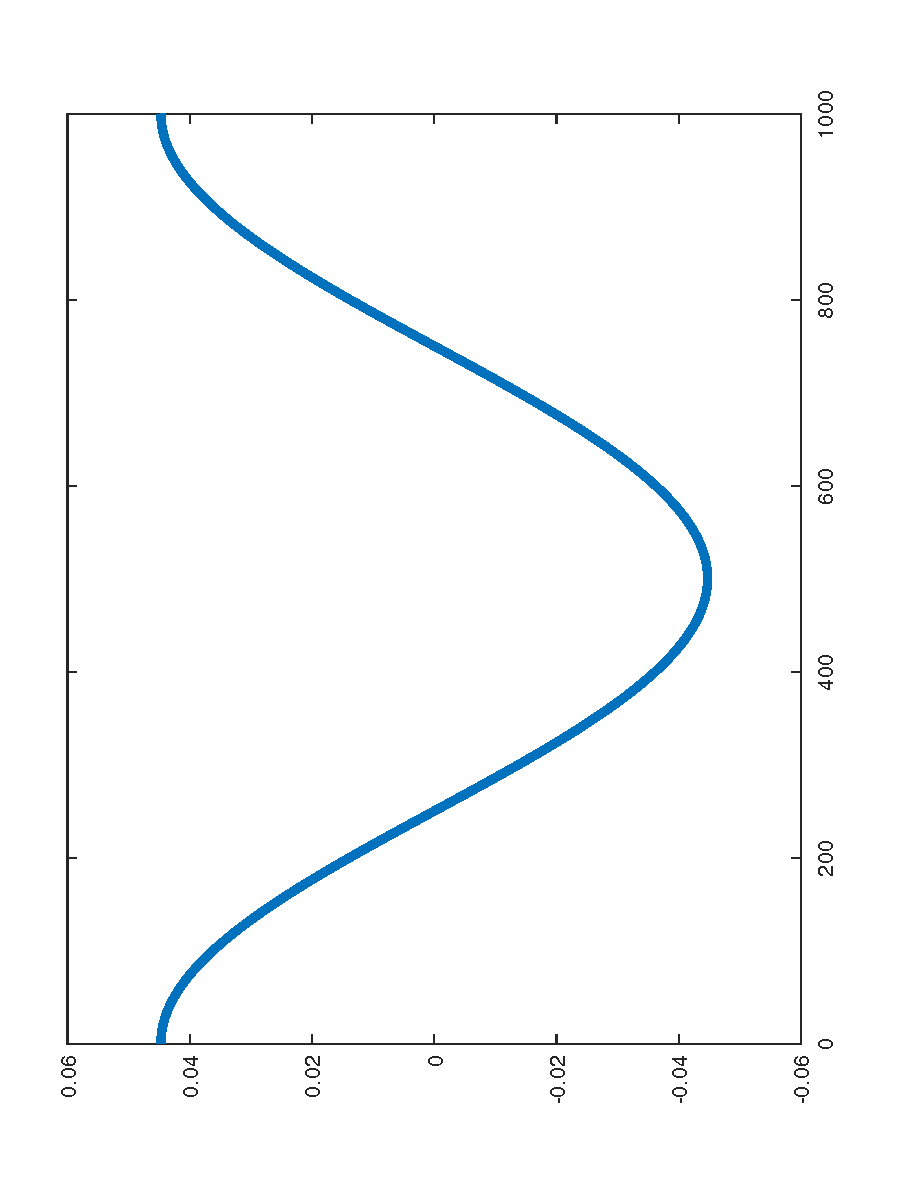
\includegraphics[
        angle=-90,
        origin=c,
        width=\textwidth]{papers/sgwt/images/line-chi-3.pdf}
        \vspace{-45pt}
        \caption{$\chi_2$ eines ungewichteten Liniengraphen mit 1000 
        Knoten.}
        \label{fig:sgwt:chi:line2}
    \end{minipage}
    ~
    \begin{minipage}[b]{0.49\textwidth}
        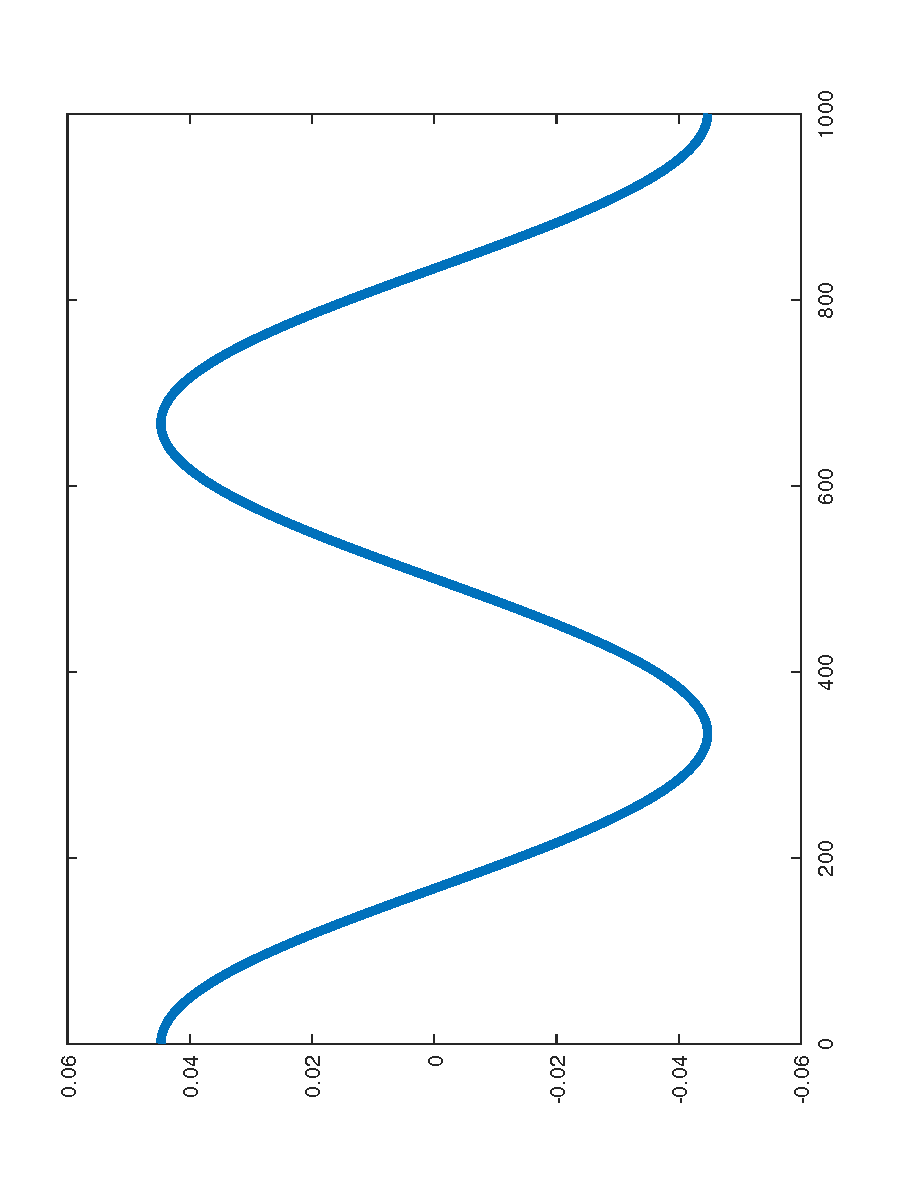
\includegraphics[
        angle=-90,
        origin=c,
        width=\textwidth]{papers/sgwt/images/line-chi-4.pdf}
        \vspace{-45pt}
        \caption{$\chi_3$ eines ungewichteten Liniengraphen mit 1000 
        Knoten.}
        \label{fig:sgwt:chi:line3}
    \end{minipage}
    ~
    \begin{minipage}[b]{0.49\textwidth}
        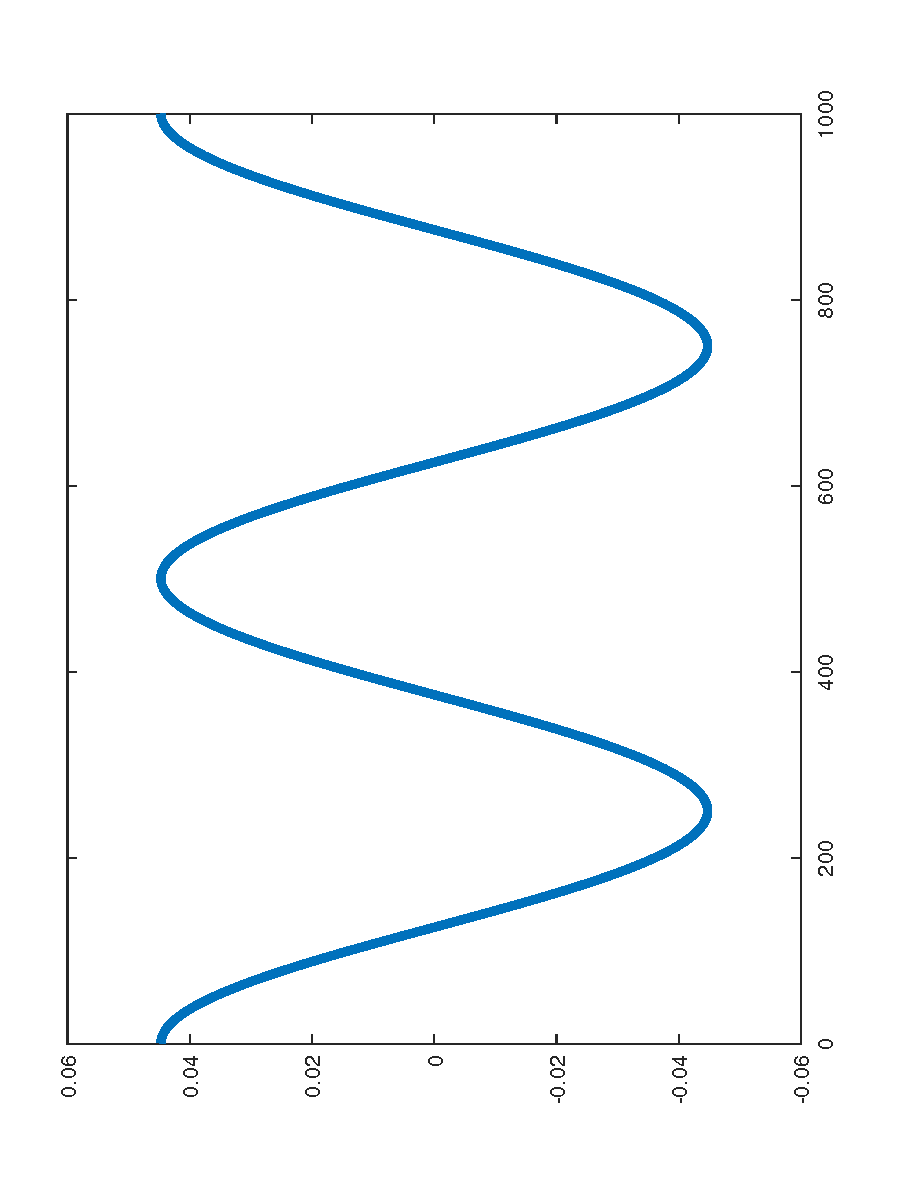
\includegraphics[
        angle=-90,
        origin=c,
        width=\textwidth]{papers/sgwt/images/line-chi-5.pdf}
        \vspace{-45pt}
        \caption{$\chi_4$ eines ungewichteten Liniengraphen mit 1000 
        Knoten.}
        \label{fig:sgwt:chi:line4}
    \end{minipage}
    ~
    \begin{minipage}[b]{0.49\textwidth}
        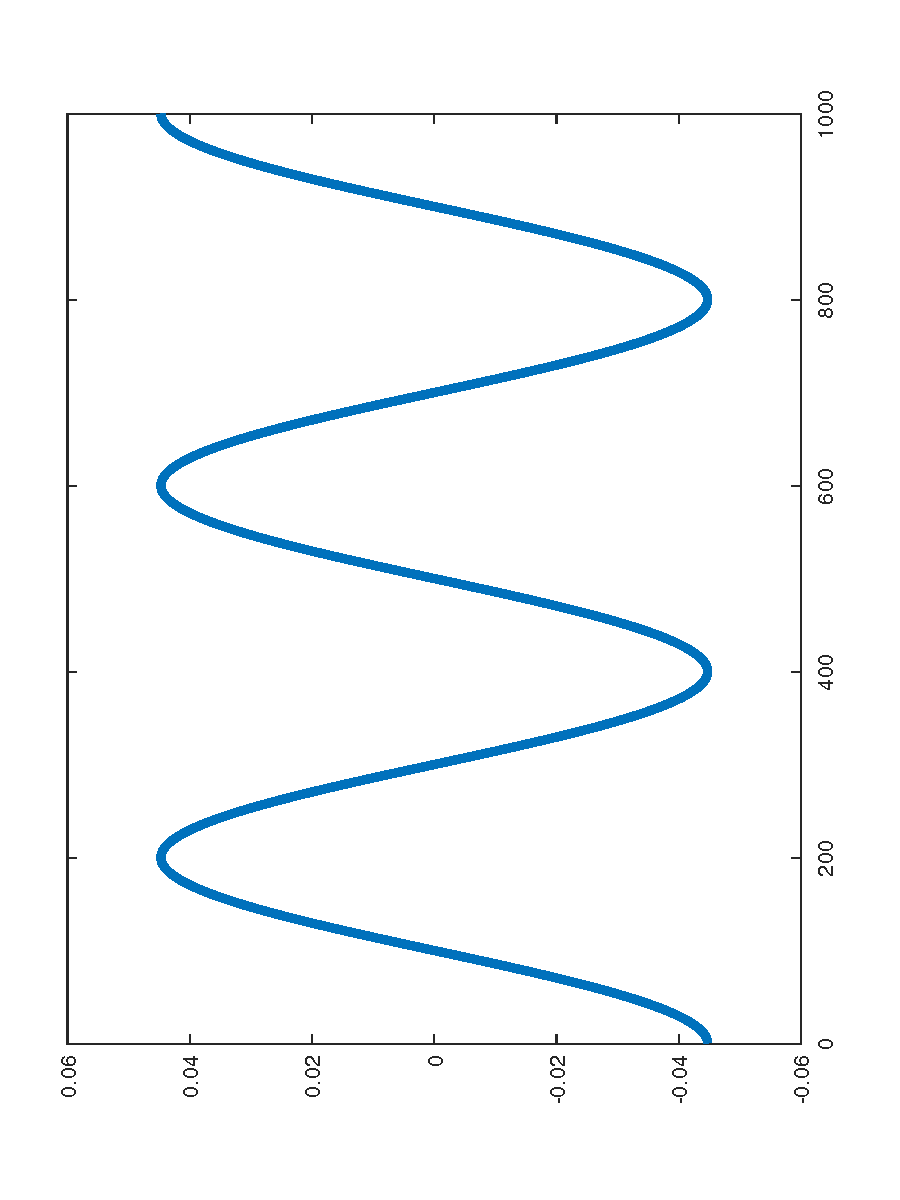
\includegraphics[
        angle=-90,
        origin=c,
        width=\textwidth]{papers/sgwt/images/line-chi-6.pdf}
        \vspace{-45pt}
        \caption{$\chi_5$ eines ungewichteten Liniengraphen mit 1000 
        Knoten.}
        \label{fig:sgwt:chi:line5}
    \end{minipage}
\end{figure}

\begin{figure}
    \centering
    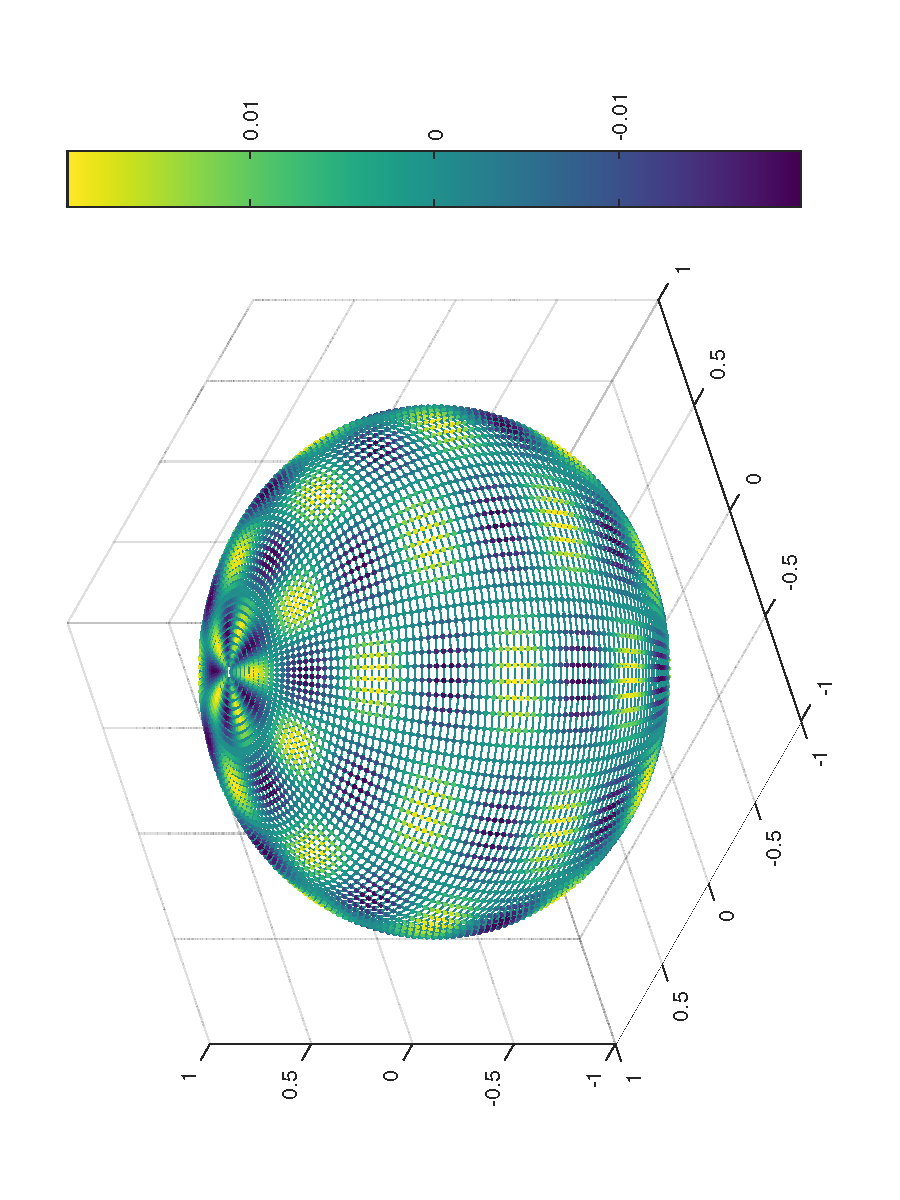
\includegraphics[
    angle=-90,
    origin=c,
    scale=0.7
    ]{papers/sgwt/images/graph-100-100-chi-150.pdf}
    \vspace{-80pt}
    \caption{Kugelgraph mit 10002 Knoten. Darstellung von $\chi_{150}$.
        \label{fig:sgwt:chi:sphere}}
\end{figure}